\documentclass[12pt]{article}

\usepackage{xcolor}
\usepackage{listings}
\usepackage{hyperref}
\usepackage{pdfpages}

\hypersetup{
    colorlinks=true,
    linkcolor=blue,
    filecolor=magenta,      
    urlcolor=cyan,
    pdftitle={HW07},
    pdfpagemode=FullScreen,
    }
\lstset{basicstyle=\ttfamily,
showstringspaces=false,
commentstyle=\color{red},
keywordstyle=\color{blue}
}

\renewcommand{\thesubsection}{\thesection.\alph{subsection}}

\title{Programming Assignment 7 \\ \small{ECE 759, Prof. TW Huang}}
\author{Sai Tadinada}
\date{}

\begin{document}
\maketitle

GitHub link to programming tasks: \\ \url{} % TODO: Add link here

\section{Question 1}

\subsection{}
\texttt{task1.cu} can be found at \url{} % TODO: Add link here

\subsection{}
Scaling analysis plot for task1 is shown below:
% \begin{figure}[ht]
% \centering
% 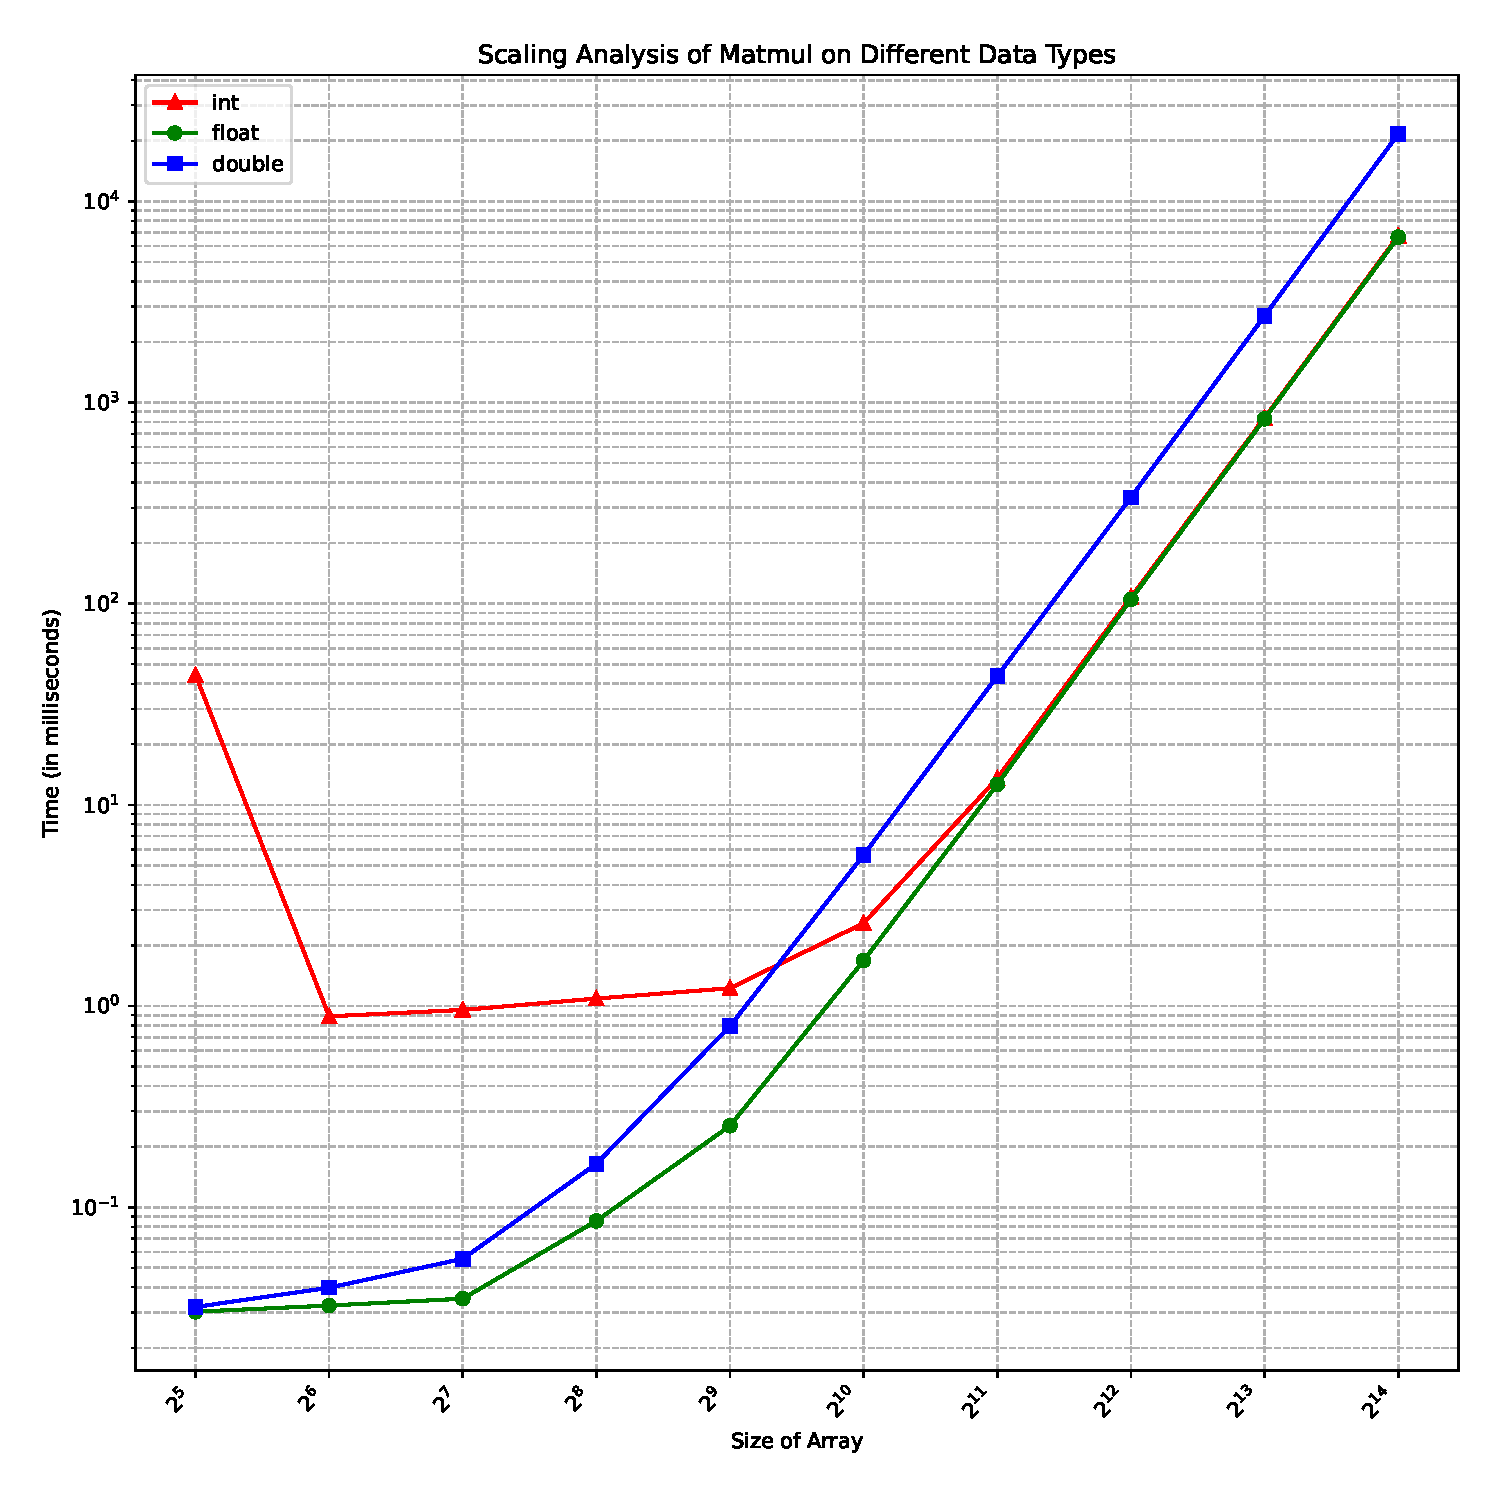
\includegraphics[width=0.8\textwidth]{task1.pdf}
% \caption{Scaling Analysis for task1 (matrix multiplication)}
% \end{figure}

\subsection{}
\subsection{} % best possible value of block_dim for n = 2^14
\subsection{} % performance change betweeen types of data
\subsection{} % CPU vs GPU of matmul on n = 2^14

\section{Question 2}

\subsection{}
\texttt{task2.cu} can be found at \url{} % TODO: Add link here

\subsection{}
Scaling analysis plot for task2 is shown below:
% \begin{figure}[ht]
% \centering
% 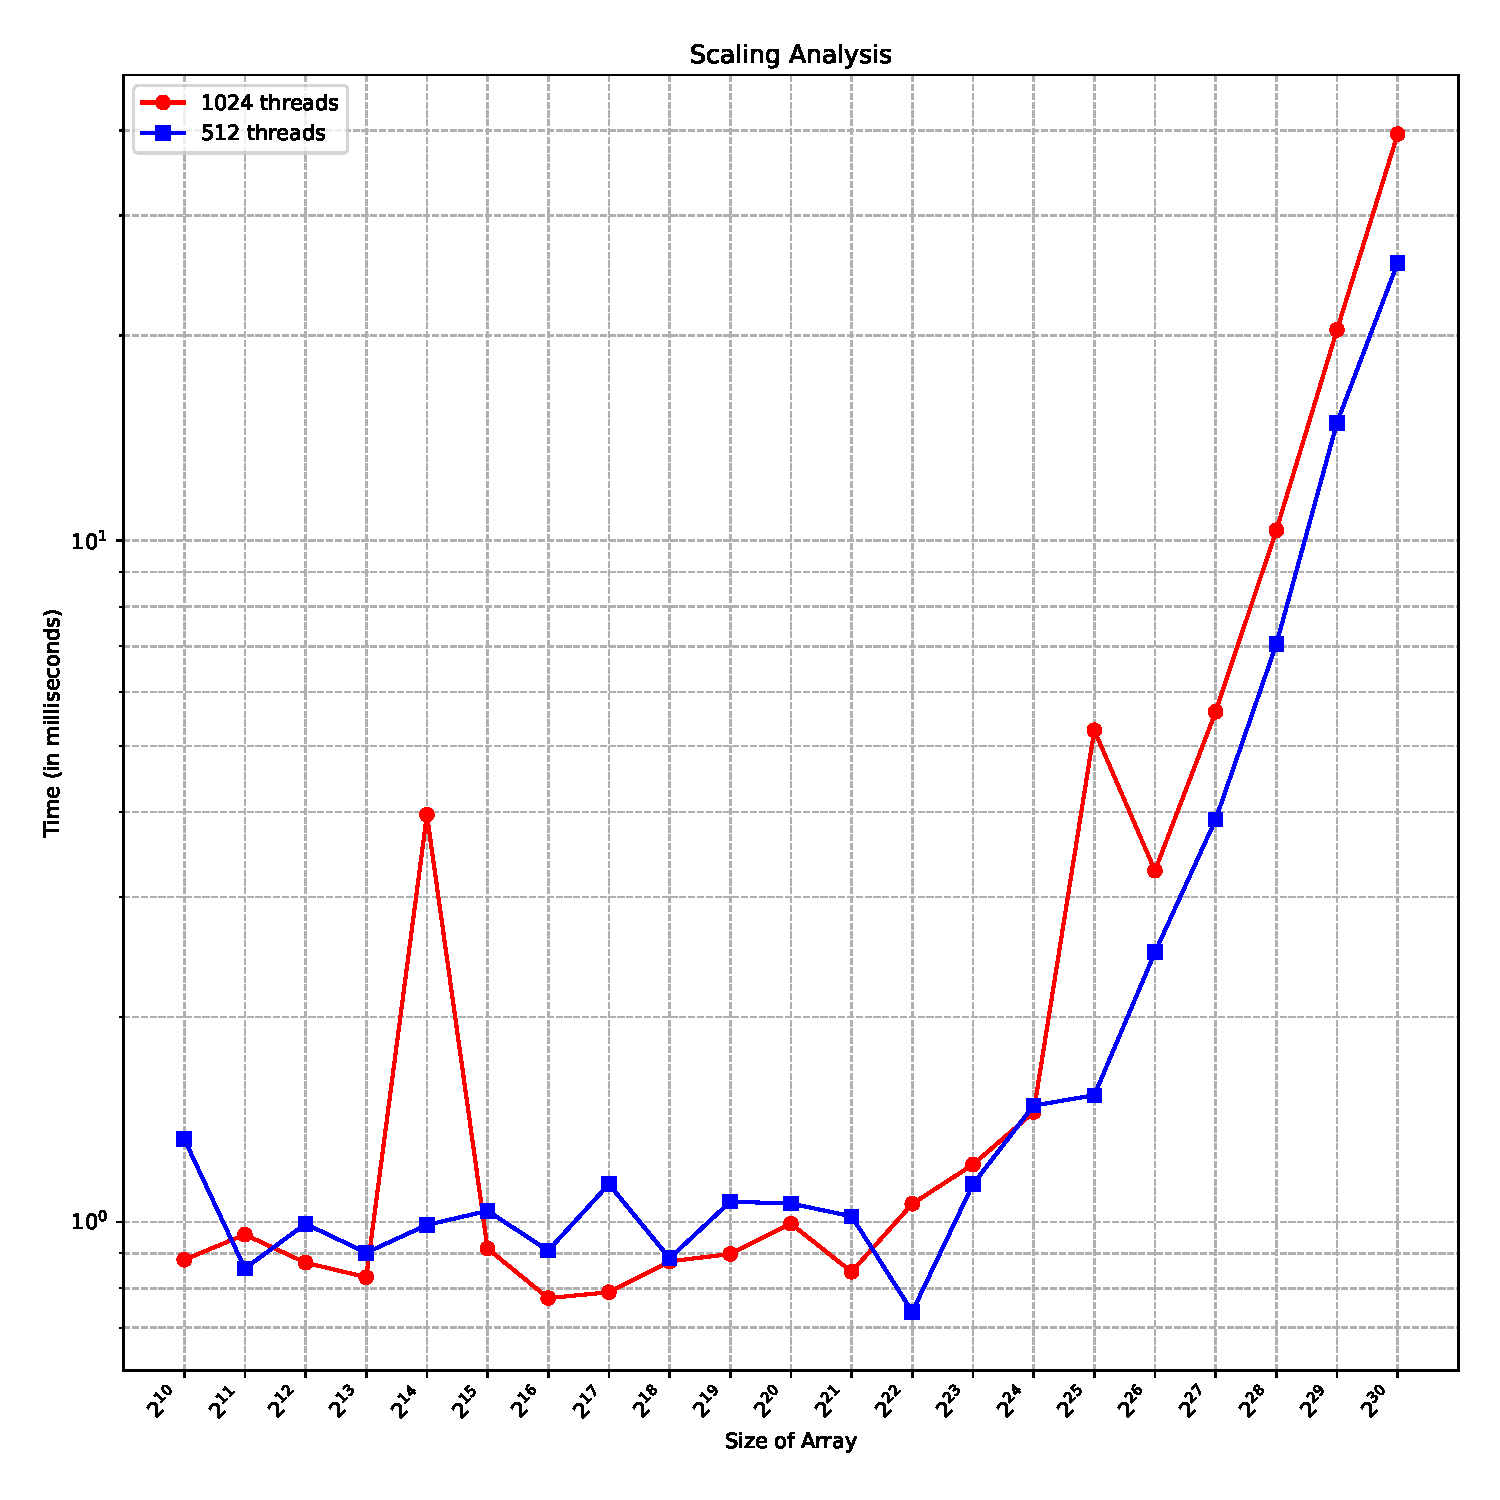
\includegraphics[width=0.7\textwidth]{task2.pdf}
% \caption{Scaling Analysis for task2 (stencil computation)}
% \end{figure}


\end{document}